\section{Link Analysis}

Will a wireless link from $A$ to $B$ work? What speeds can be
expected? How much transmit power is necessary and what kind of
antennae should be used? To answer these questions we do a link budget
calculation. This is,
\begin{equation}
  \label{eq:link_budget}
  P_r = P_t + G + L
\end{equation}
or, the received power is equal to the transmit power, plus gains, and
minus losses. We then check in the manufacturer's table to see if the
received power is sufficient to maintain a link and at what speed.

The main difficulty is in figuring out what $L$ is, because there are
lots of different sources of loss, for example:
\begin{itemize}
  \item cable loss caused by electrical resistance of a feedline
    between  between the radio and the antenna
  \item insertion loss caused by the use of connectors to attach the
    feedline
  \item path loss caused by the spreading out of energy in space (this
    is your ``inverse-$r^2$'' loss)
  \item path loss related to the decreasing ability of an antenna to
    ``hear'' radio waves as the frequency increases (this loss is
    proportional to the square of the frequency)
  \item multi-path loss where two signals from
    the same transmitter follow different paths to the receiver and
    interfere destructively with one another
  \item absorption, primarily by water in the air such as rain and
    fog, but also at higher frequencies by elements such as oxygen and
    nitrogen an effect which varies depending on frequency.
\end{itemize}

To see how this works, let us take a specific example, the link from
Eigg to Ranachan and supposing that the link was to be done with our
common Ubiquiti Rocket M5 radios and dishes. 

\begin{figure}[h]
  \begin{center}
    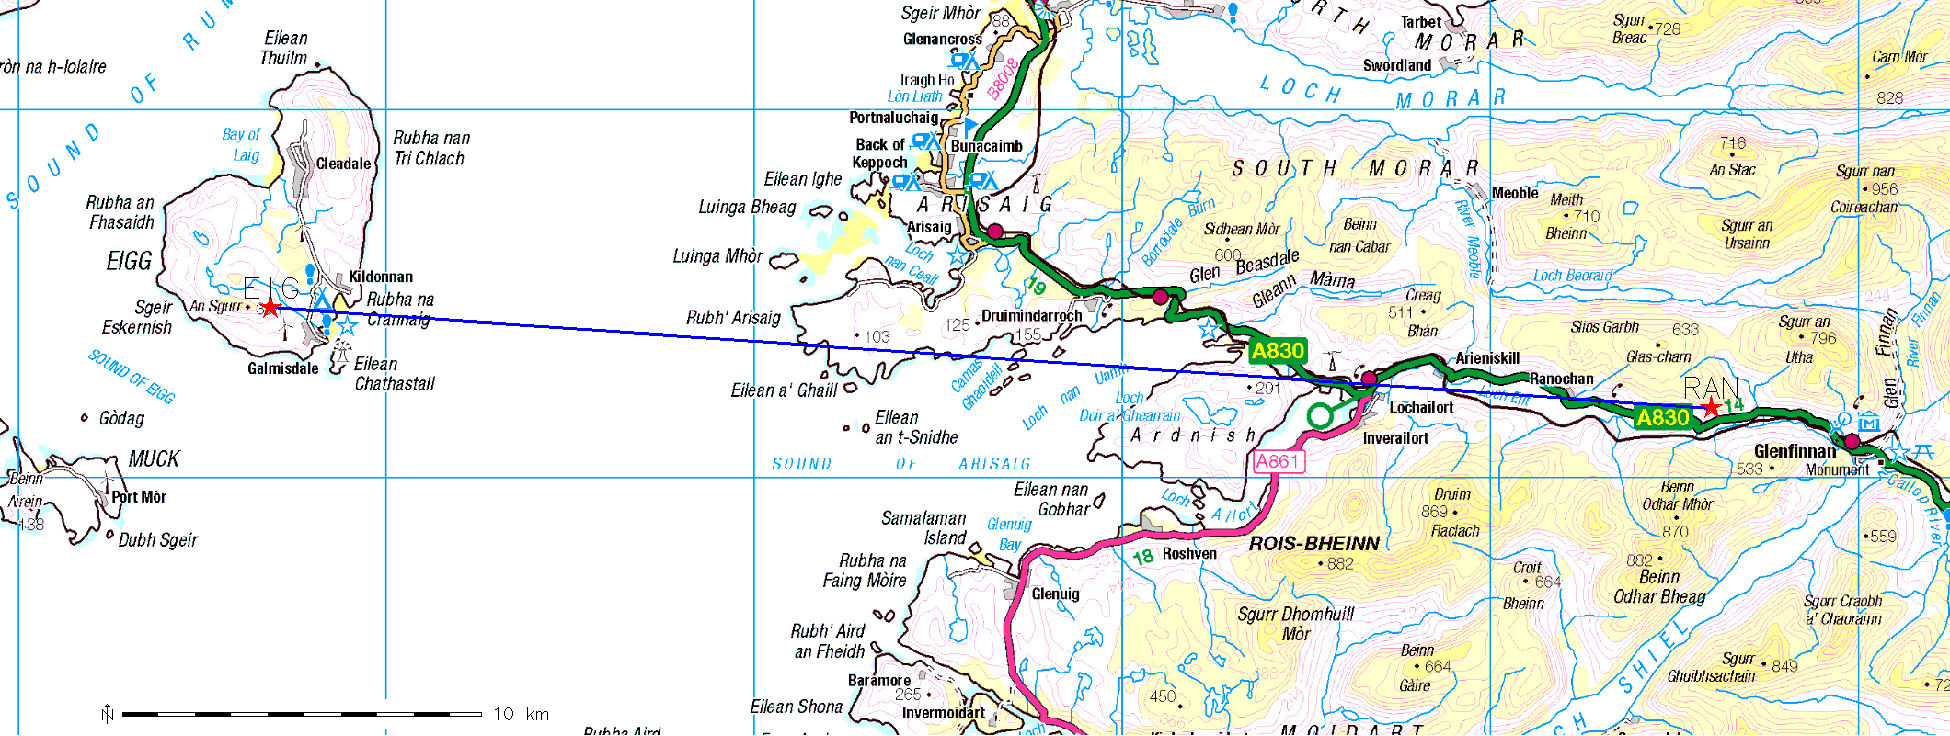
\includegraphics[width=\textwidth]{special/EIG_RAN_map.png}
  \end{center}
  \caption{Map of the Eigg to Ranachan path}
  \label{fig:eig_ran_map}
\end{figure}

Figure \ref{fig:eig_ran_map} gives an idea of what we're trying to
accomplish, a link between two places about 40km apart (actually it
turns out that they're almost exactly that distance). So the first
question is, all else being equal, in a vacuum in outer space, can we
use these radios to make a 40km link at 5GHz?

\subsection{Path Loss}
In outer space we have only path loss, which is given by
\begin{equation}
L_p = 20 \log \left(\frac{\lambda}{4 \pi R}\right)
\end{equation}
this can be derived, but it's a bit tricky and we won't do it
here. Just observe the general shape of it. The $2$ is because in
non-logarithmic form everything in the brackets is squared. We use the
logarithmic form because it means we can just add things up instead of
multiplying which is easier. The $10$ (from $2 \times 10 = 20$) is
because the numbers are all in decibels (dB), this is just convention,
but we need to be consistent. The $1/R$ is the inverse-$r^2$
loss from the radio waves spreading out in space, and the $\lambda$ is
because antennas get relatively more deaf as the wavelength gets
smaller. That's it apart from some constants that basically come from
the geometry involved.

We know the frequency (pick the middle of the band, for example) and
the speed of light, and we can work out that
\begin{equation}
\lambda = \frac{c}{f}
\end{equation}
or in this case
$$
\lambda = \frac{%
  300,000,000\, \mathrm{m}/\mathrm{s}%
}{%
  5,650,000,000\,\mathrm{hz}%
} = 0.053\, \mathrm{m}
$$

This is now enough to just directly work out $L_p$ with the help of a
pocket calculator,
$$
L_p = 20 \times \log \left( \frac{0.053}{4 \times \pi \times 40000} \right)
= -140\,\mathrm{dB}
$$

This loss is what we have to overcome assuming everything else is
perfect and ideal and lossless. Suppose we (illegally) run our Rocket
radios at the maximum output power ($27\,\mathrm{dBm}$) and use the
run of the mill $30\, \mathrm{dBi}$ dishes on either end. Putting these
numbers into our link budget equation \ref{eq:link_budget}, we get:
$$
P_r = 27 + 30 + 30 - 140 = -53\, \mathrm{dBm}
$$

\subsection{Transmit Power and Receive Sensitivity}
So that's pretty good, but to interpret this better we now have to
look at the datasheet for the radio. The relevant numbers are
reproduced in figure \ref{fig:rocket_txrx}.
\begin{figure}[h]
  \begin{center}
    \begin{tabular}{lrrr}
      Modulation & Line rate & TX power & RX sensitivity\\
      \hline
      MCS0 & $6.5\, \mathrm{Mbps}$ & $27\, \mathrm{dBm}$ & $-96\,\mathrm{dBm}$\\
      MCS1 & $13\, \mathrm{Mbps}$ & $27\, \mathrm{dBm}$ & $-95\,\mathrm{dBm}$\\
      MCS2 & $19.5\, \mathrm{Mbps}$ & $27\, \mathrm{dBm}$ & $-92\,\mathrm{dBm}$\\
      MCS3 & $26\, \mathrm{Mbps}$ & $27\, \mathrm{dBm}$ & $-90\,\mathrm{dBm}$\\
      MCS4 & $39\, \mathrm{Mbps}$ & $26\, \mathrm{dBm}$ & $-86\,\mathrm{dBm}$\\
      MCS5 & $52\, \mathrm{Mbps}$ & $24\, \mathrm{dBm}$ & $-83\,\mathrm{dBm}$\\
      MCS6 & $58.5\, \mathrm{Mbps}$ & $22\, \mathrm{dBm}$ & $-77\,\mathrm{dBm}$\\
      MCS7 & $65\, \mathrm{Mbps}$ & $21\, \mathrm{dBm}$ & $-74\,\mathrm{dBm}$\\
      MCS8 & $13\, \mathrm{Mbps}$ & $27\, \mathrm{dBm}$ & $-95\,\mathrm{dBm}$\\
      MCS9 & $26\, \mathrm{Mbps}$ & $27\, \mathrm{dBm}$ & $-93\,\mathrm{dBm}$\\
      MCS10 & $39\, \mathrm{Mbps}$ & $27\, \mathrm{dBm}$ & $-90\,\mathrm{dBm}$\\
      MCS11 & $52\, \mathrm{Mbps}$ & $27\, \mathrm{dBm}$ & $-87\,\mathrm{dBm}$\\
      MCS12 & $78\, \mathrm{Mbps}$ & $26\, \mathrm{dBm}$ & $-84\,\mathrm{dBm}$\\
      MCS13 & $104\, \mathrm{Mbps}$ & $24\, \mathrm{dBm}$ & $-79\,\mathrm{dBm}$\\
      MCS14 & $117\, \mathrm{Mbps}$ & $22\, \mathrm{dBm}$ & $-78\,\mathrm{dBm}$\\
      MCS15 & $130\, \mathrm{Mbps}$ & $21\, \mathrm{dBm}$ & $-75\,\mathrm{dBm}$\\
    \end{tabular}
  \end{center}
  \caption{Transmit power and receive sensitivity for Ubiquiti Rocket
    M5 at different modulation rates. All $\mathrm{dBm}$ values are
    $+/-\, 2\, \mathrm{dB}$}
  \label{fig:rocket_txrx}
\end{figure}

A few observations about these figures. When using these radios with
dual-polarised antennas, we will never see the MCS0-MCS7 modulation
schemes because these are for single data streams. So the only ones of
interest are MCS8-MCS15. The transmit power that the radios are
capable of is less at the higher modulations. For example if we want
full speed, we can only transmit at $21\, \mathrm{dBm}$ -- that's four
times weaker than at full power (because $10^{0.3} \approx 2$). 

Supposing that we want as fast as possible a link, we need to adjust
our calculation above setting $P_t = 21$ and so we now get
$P_r = -59\, \mathrm{dBm}$.

Also, the receive sensitivty for the slower rates is really very good,
better than $-90\, \mathrm{dBm}$. In practice we will never see links
established with signal strengths at or near that range because of
ambient noise -- which tends to be at about that level.

The meaning of the receive sensitivity is that the receiver part of
the radio needs a signal at least that strong in order to establish a
connection at a given data rate. So we have calculated that we should
see a $P_r$ of $-59\, \mathrm{dBm}$ and we only need $-75\, \mathrm{dBm}$.
That's pretty good, there's a margin of $16\, \mathrm{dB}$ and all
else being equal the link should work.

Actually $16\, \mathrm{dB}$ is fairly thin. \textbf{Typically a margin
  of $20-25\, \mathrm{dB}$ is used to be confident that a link will
  work well}. Remember that dishes move in the wind, alignment never
stays perfect, though manufacturing quality is generally pretty good,
it isn't perfect. The response of the antennas is not flat over their
entire operating range and they can never be absolutely perfectly
matched. There are also cable and connector losses at either end that
might run to $1.5\, \mathrm{dB}$.

\subsection{Regulatory Limits}

But then we remember. In the UK, the power limits for the upper part
of the $5\,\mathrm{GHz}$ band are $36\, \mathrm{dBm}$. That means with
a $30\, \mathrm{dBi}$ dish, we are only allowed to run the transmitter
at $6\, \mathrm{dBm}$ not $21$. That has just eaten up our entire
margin!

So, how long a link can we do \textit{legally}? We have enough
information to work this out. Assuming a $20\, \mathrm{dB}$ margin, we
know that,
$$
-75 + 20 = 6 + 30 + 30 + 20 \times
\log \left(\frac{0.053}{4 \times \pi \times R} \right)
$$
rearranging,
$$
R = \frac{%
  0.053
}{%
  4 \times \pi \times 10^{\left(-75 + 20 - 6 - 30 - 30\right)/20}%
} = 4732\, \mathrm{m}
$$

Yes, that's $4.7\, \mathrm{km}$. Using bigger $34\, \mathrm{dBi}$
dishes improves this to about $7.5\, \mathrm{km}$. With a thinner
margin and tolerating a lower data rate at MCS12, we can eak out close
to $25\, \mathrm{km}$. Using the normal dishes, the best we can hope
for is about $15\, \mathrm{km}$ Any longer than that, and rules are
definitely being broken. And the link that we are considering is more
than twice the best that we could possibly do.

\subsection{Fresnel Zones}

\begin{figure}[h]
  \begin{center}
    % GNUPLOT: LaTeX picture with Postscript
\begingroup
  \makeatletter
  \providecommand\color[2][]{%
    \GenericError{(gnuplot) \space\space\space\@spaces}{%
      Package color not loaded in conjunction with
      terminal option `colourtext'%
    }{See the gnuplot documentation for explanation.%
    }{Either use 'blacktext' in gnuplot or load the package
      color.sty in LaTeX.}%
    \renewcommand\color[2][]{}%
  }%
  \providecommand\includegraphics[2][]{%
    \GenericError{(gnuplot) \space\space\space\@spaces}{%
      Package graphicx or graphics not loaded%
    }{See the gnuplot documentation for explanation.%
    }{The gnuplot epslatex terminal needs graphicx.sty or graphics.sty.}%
    \renewcommand\includegraphics[2][]{}%
  }%
  \providecommand\rotatebox[2]{#2}%
  \@ifundefined{ifGPcolor}{%
    \newif\ifGPcolor
    \GPcolortrue
  }{}%
  \@ifundefined{ifGPblacktext}{%
    \newif\ifGPblacktext
    \GPblacktexttrue
  }{}%
  % define a \g@addto@macro without @ in the name:
  \let\gplgaddtomacro\g@addto@macro
  % define empty templates for all commands taking text:
  \gdef\gplbacktext{}%
  \gdef\gplfronttext{}%
  \makeatother
  \ifGPblacktext
    % no textcolor at all
    \def\colorrgb#1{}%
    \def\colorgray#1{}%
  \else
    % gray or color?
    \ifGPcolor
      \def\colorrgb#1{\color[rgb]{#1}}%
      \def\colorgray#1{\color[gray]{#1}}%
      \expandafter\def\csname LTw\endcsname{\color{white}}%
      \expandafter\def\csname LTb\endcsname{\color{black}}%
      \expandafter\def\csname LTa\endcsname{\color{black}}%
      \expandafter\def\csname LT0\endcsname{\color[rgb]{1,0,0}}%
      \expandafter\def\csname LT1\endcsname{\color[rgb]{0,1,0}}%
      \expandafter\def\csname LT2\endcsname{\color[rgb]{0,0,1}}%
      \expandafter\def\csname LT3\endcsname{\color[rgb]{1,0,1}}%
      \expandafter\def\csname LT4\endcsname{\color[rgb]{0,1,1}}%
      \expandafter\def\csname LT5\endcsname{\color[rgb]{1,1,0}}%
      \expandafter\def\csname LT6\endcsname{\color[rgb]{0,0,0}}%
      \expandafter\def\csname LT7\endcsname{\color[rgb]{1,0.3,0}}%
      \expandafter\def\csname LT8\endcsname{\color[rgb]{0.5,0.5,0.5}}%
    \else
      % gray
      \def\colorrgb#1{\color{black}}%
      \def\colorgray#1{\color[gray]{#1}}%
      \expandafter\def\csname LTw\endcsname{\color{white}}%
      \expandafter\def\csname LTb\endcsname{\color{black}}%
      \expandafter\def\csname LTa\endcsname{\color{black}}%
      \expandafter\def\csname LT0\endcsname{\color{black}}%
      \expandafter\def\csname LT1\endcsname{\color{black}}%
      \expandafter\def\csname LT2\endcsname{\color{black}}%
      \expandafter\def\csname LT3\endcsname{\color{black}}%
      \expandafter\def\csname LT4\endcsname{\color{black}}%
      \expandafter\def\csname LT5\endcsname{\color{black}}%
      \expandafter\def\csname LT6\endcsname{\color{black}}%
      \expandafter\def\csname LT7\endcsname{\color{black}}%
      \expandafter\def\csname LT8\endcsname{\color{black}}%
    \fi
  \fi
  \setlength{\unitlength}{0.0500bp}%
  \begin{picture}(8280.00,8640.00)%
    \gplgaddtomacro\gplbacktext{%
      \csname LTb\endcsname%
      \put(946,1636){\makebox(0,0)[r]{\strut{}-50}}%
      \put(946,2366){\makebox(0,0)[r]{\strut{} 0}}%
      \put(946,3095){\makebox(0,0)[r]{\strut{} 50}}%
      \put(946,3824){\makebox(0,0)[r]{\strut{} 100}}%
      \put(946,4554){\makebox(0,0)[r]{\strut{} 150}}%
      \put(946,5283){\makebox(0,0)[r]{\strut{} 200}}%
      \put(946,6012){\makebox(0,0)[r]{\strut{} 250}}%
      \put(946,6742){\makebox(0,0)[r]{\strut{} 300}}%
      \put(946,7471){\makebox(0,0)[r]{\strut{} 350}}%
      \put(946,8201){\makebox(0,0)[r]{\strut{} 400}}%
      \put(1240,1144){\makebox(0,0){\strut{} 0}}%
      \put(2065,1144){\makebox(0,0){\strut{} 5000}}%
      \put(2891,1144){\makebox(0,0){\strut{} 10000}}%
      \put(3716,1144){\makebox(0,0){\strut{} 15000}}%
      \put(4542,1144){\makebox(0,0){\strut{} 20000}}%
      \put(5367,1144){\makebox(0,0){\strut{} 25000}}%
      \put(6192,1144){\makebox(0,0){\strut{} 30000}}%
      \put(7018,1144){\makebox(0,0){\strut{} 35000}}%
      \put(7843,1144){\makebox(0,0){\strut{} 40000}}%
      \put(176,4869){\rotatebox{-270}{\makebox(0,0){\strut{}Elevation (meters)}}}%
      \put(4480,814){\makebox(0,0){\strut{}Distance (meters)}}%
      \put(1240,2016){\makebox(0,0)[l]{\strut{}Path length:}}%
      \put(2601,2016){\makebox(0,0)[l]{\strut{}39261 meters}}%
      \put(1240,1806){\makebox(0,0)[l]{\strut{}Frequency:}}%
      \put(2601,1806){\makebox(0,0)[l]{\strut{}5650 MHz}}%
      \put(1240,1595){\makebox(0,0)[l]{\strut{}Path loss:}}%
      \put(2601,1595){\makebox(0,0)[l]{\strut{}-139 dB}}%
    }%
    \gplgaddtomacro\gplfronttext{%
      \csname LTb\endcsname%
      \put(3454,393){\makebox(0,0)[r]{\strut{}Elevation Profile}}%
      \csname LTb\endcsname%
      \put(3454,173){\makebox(0,0)[r]{\strut{}First Fresnel Zone}}%
      \csname LTb\endcsname%
      \put(6685,393){\makebox(0,0)[r]{\strut{}Direct path}}%
    }%
    \gplbacktext
    \put(0,0){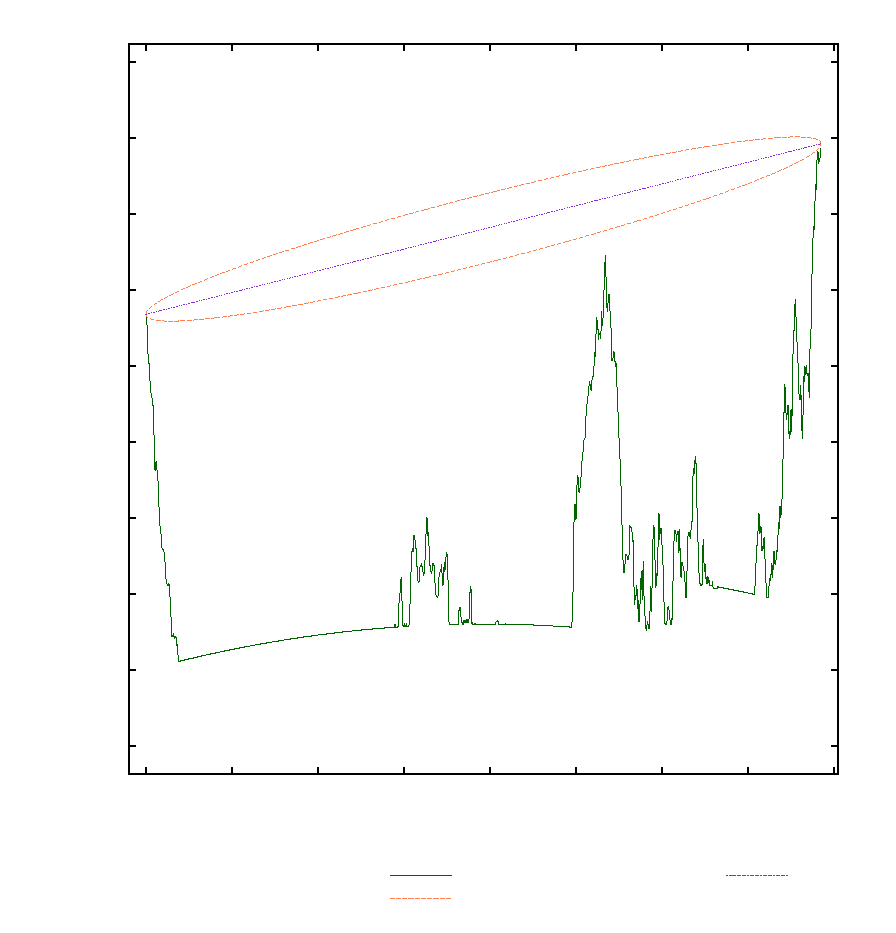
\includegraphics{special/EIG_RAN}}%
    \gplfronttext
  \end{picture}%
\endgroup

    \caption{Path profile, Eigg $\rightarrow$ Ranachan}
    \label{fig:EIG_RAN_profile}
  \end{center}
\end{figure}

So now that we have a reasonable handle on the links themselves, lets
put them into context. Figure \ref{fig:EIG_RAN_profile} shows what the
path looks like from the side. The profile of the sea and the hills is
corrected for the curvature of the earth, which matters.

It is important that there are no obstruction. Rock and, to a lesser
extent trees and vegetation causes extremely high loss. A signal is
unlikely to travel more than a meter or so through rock and
considerably less if the iron content is high.

It is also important that not only the direct path itself is clear but
that there is nothing nearby that could cause reflections that will
interfere with the direct signal. Reflections will interfere
destructively if they are out of phase with the original signal, and
constructively if they are in phase. As the reflector is moved away
from the direct path, reflections will at first be destructive and
then become constructive, and then destructive again and so forth. The
boundaries between these zones are called Fresnel Ellipsoids and the
zones themselves are called Fresnel Zones.

In practice we only worry about the first Fresnel Zone, and the second
one is beneficial to us. The first zone must be kept clear, if it is
obstructed then we have to worry about additional loss caused by
destructive interference. The oval shape in figure
\ref{fig:EIG_RAN_profile} is the first such zone, and in this case we
are in good shape. Particularly so because the peak in the
centre-right of the picture will do two things. First it is in the
second Fresnel Zone so anything reflected off the top of it can only
help, and secondly any reflections from lower down in the
$3^\mathrm{rd}$, $5^\mathrm{th}$ etc zones will be blocked by that
hill itself and will never reach the receiver to interfere.

\subsection{Rain Fade}

All the previous sections on link budgets and loss apply at pretty
much every frequency. Lower frequencies can go farther with the same
power and gain, Fresnel Zones are thinner at higher frequencies, but
the effects and the calculations are exactly the same. There is,
however, an important phenomenon that starts to come into play at
higher frequencies -- attenuation by water in the air. In other words,
rain. The higher the frequency the more this matters and needs to be
explicitly taken into account starting at around $6\, \mathrm{GHz}$. 

Figure \ref{fig:rain_fade} lists the attenuation that can be expected
at different frequencies, at different rates of rain.  The numbers are
rough, being read off a chart in a report published in the 1970s by
the Rand Corporation for the US Air Force, but they should be fairly
accurate.

\begin{figure}
  \begin{center}
    \begin{tabular}{l|rrrr}
      $rain\backslash f$ & $6$ & $11$ & $18$ & $23$ \\
      \hline
      $2.5$ & $< 0.1$ & $< 0.1$ & $0.1$ & $0.3$\\
      $5$   & $< 0.1$ & $0.1$ & $0.3$ & $0.9$\\ 
      $12.5$ & $< 0.1$ & $0.6$ & $1.5$ & $3$\\
      $25$ & $0.1$ & $1.5$ & $3$ & $5$\\
      $50$ & $0.5$ & $3$ & $7$ & $9$\\
    \end{tabular}
  \end{center}
  \caption{Attenuation by rain. Rain values are in mm/hr, frequencies
    in GHz. Values in the table are dB/km.}
  \label{fig:rain_fade}
\end{figure}

It is easy to see that even very heavy rain does not affect the
$6\,\mathrm{GHz}$ band very much. On the other hand even moderately
heavy rain can badly affect a $23\, \mathrm{GHz}$ link. This is one
reason why licenses for the higher frequencies are cheaper than for
the lower ones. At higher frequencies, a rainy day can easily
attenuate a signal on a short $5\, \mathrm{km}$ link by maybe $15\,
\mathrm{dB}$ which will seriously impact its performance. Longer links
at high frequencies are just not feasible.

In Scotland we should budget for $15\, \mathrm{mm/hr}$ of rain inland,
$20\, \mathrm{mm/hr}$ of rain in coastal areas and $25\,\mathrm{mm/hr}$
in the Outer Isles.

